\section{Data Quality and Diagnostics}
\label{sec:si_diagnostics}

\begin{figure}[H]
 \centering
 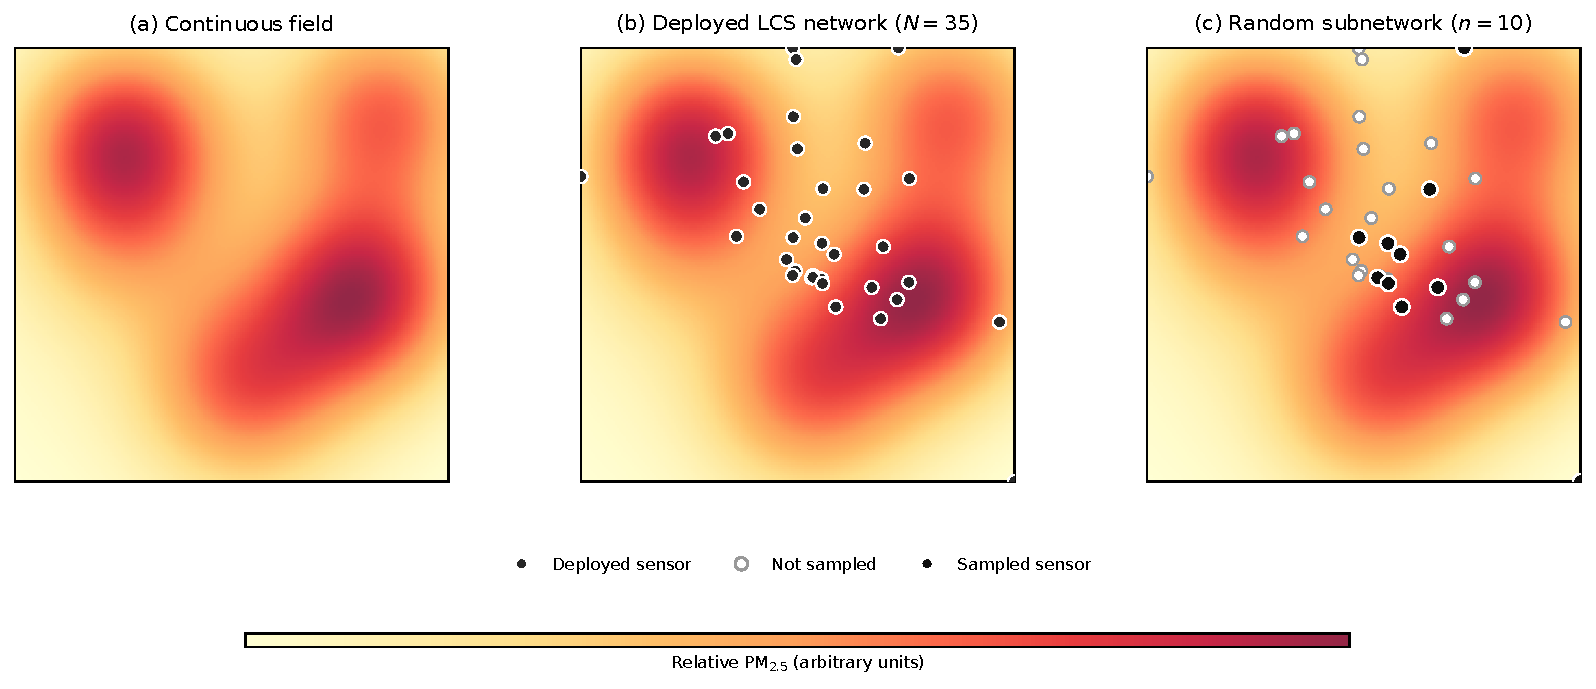
\includegraphics[width=0.95\textwidth]{Plots/Supporting_Information/Figure_SI_12/estimand_schematic.pdf}
 \caption{Estimand schematic. \textbf{(a)} The true, continuous \pmtt\ field is unobserved and is \emph{not} the target of this study; the field shown here is hypothetical (relative, arbitrary units). \textbf{(b)} The deployed low-cost-sensor network (here $N=35$) defines the estimand: the reference-network mean $\mu_{\mathrm{ref}}$, the arithmetic mean of the deployed sensor means. \textbf{(c)} A simple random subnetwork of $n$ sensors (here $n=10$) gives the subnetwork mean $\widehat{\mu}_{n}$, whose accuracy we quantify by the absolute percentage error $\mathrm{APE}=\lvert\widehat{\mu}_{n}-\mu_{\mathrm{ref}}\rvert/\mu_{\mathrm{ref}}\times100\%$. The schematic fixes the central framing of the study: the estimand is the deployed reference-network mean---not the true continuous field, nor an area- or population-weighted city mean.}
 \label{fig:si_estimand_schematic}
\end{figure}

This Supporting Information section summarizes the diagnostic checks performed on the finalized \pmtt\ datasets used in the main analysis. \city{Dhaka} and \city{Lucknow} use processed hourly data for April~2022--March~2023, whereas \city{Chicago} uses the Open Air official daily calibrated aggregate for September~2025--May~2026, with hourly-derived diagnostics used only for sensitivity analyses. The deployment teams implemented QA/QC screening, calibration, and within-network harmonization prior to aggregation. Our goal here is to characterize data completeness, internal consistency, and potential anomaly patterns in the processed time series, and to document what was (and was not) enforced in downstream analysis.

\begin{itemize}
 \item \textbf{Completeness (post QA/QC):} After the QA/QC screening, $85.8\%$ (\city{Dhaka}) and $71.7\%$ (\city{Lucknow}) of all possible hourly records were retained, implying missingness of $14.2\%$ and $28.3\%$, respectively. In the \city{Chicago} official daily calibrated dataset, $97.2\%$ of possible sensor-days were present after excluding collocated AQS sensors, implying missingness of $2.8\%$. Median sensor uptime was $87.6\%$ in \city{Dhaka}, $73.2\%$ in \city{Lucknow}, and $99.6\%$ in \city{Chicago}. In the main analysis, we did not impose any additional completeness rule (e.g., minimum hours per day) beyond the initial QA/QC flags and physical plausibility screening; daily and study-period means therefore use all available valid records within each aggregation window.

 \item \textbf{Within-network consistency:} We assessed agreement by correlating each sensor's series against the contemporaneous network median (rather than the mean, to reduce sensitivity to transient local spikes). Median hourly sensor-to-network correlation was $r=0.891$ in \city{Dhaka} and $r=0.950$ in \city{Lucknow}. For \city{Chicago}, the analogous official-daily correlation was $r=0.986$ [IQR: 0.980--0.989], indicating that, after calibration and harmonization, most sensors track a common network-scale temporal signal.

 \item \textbf{Anomaly scorecard (diagnostic only):} We computed an auxiliary diagnostic scorecard to identify sensors with patterns suggestive of potential artifacts. This scorecard was used for characterization and visualization, not as an additional exclusion step in the main analysis. The criteria were:
 \begin{enumerate}
 \item \textbf{Low correlation:} sensors with $r < 0.5$ against the network median;
 \item \textbf{Level shifts:} baseline changes detected using the PELT changepoint algorithm;
 \item \textbf{High spike frequency:} sensors with frequent abrupt spikes (e.g., $>5\%$ of readings, as defined in the retained diagnostic scorecard outputs).
 \end{enumerate}
\end{itemize}

\noindent No sensors in either \city{Dhaka} or \city{Lucknow} exhibited very low correlation ($r<0.5$), suggesting that no nodes were effectively disconnected from the network-scale signal in the processed dataset. The spike-frequency component of the scorecard was intentionally conservative and flagged 15 sensors in \city{Dhaka} and 38 in \city{Lucknow}. \city{Chicago}'s official-daily network coherence is summarized separately in Section~\ref{sec:si_chicago_diagnostics}. Additional inspection indicates that many flagged episodes are consistent with hyper-local transient event patterns (e.g., nearby combustion) rather than persistent hardware failure. Because the main analysis does not remove these flagged periods beyond the initial QA/QC, these diagnostics should be interpreted as describing residual local variability present in the finalized dataset rather than additional filtering. This choice reflects typical operating conditions for deployed networks; consequently, our subnetwork performance estimates incorporate realistic micro-scale variability and should be interpreted as conservative relative to an idealized setting in which such transient local influences could be perfectly identified and removed.

\paragraph{Spatial coverage.}
The sensor networks span convex-hull areas of approximately 343~km$^2$ (\city{Dhaka}), 1{,}508~km$^2$ (\city{Lucknow}), and 696~km$^2$ (\city{Chicago}), with median nearest-neighbor distances of 1.6, 1.9, and 1.4~km, respectively (Table~\ref{tab:spatial_support}). The corresponding sensor densities are 10.2, 4.7, and 39.8 sensors per 100~km$^2$ of convex hull. This broad spatial spread supports the use of the deployed-network mean as a defensible target for finite-population subnetwork experiments, while making clear that the estimand is the deployed network rather than an area- or population-weighted city mean.

\paragraph{Gap characteristics.}
Beyond overall completeness, we examined the temporal distribution of data gaps. The maximum continuous gap per sensor was 46.5~days in \city{Dhaka}, 326.7~days in \city{Lucknow} (driven by a single sensor with 4.5\% uptime), and 150~days in \city{Chicago} (driven by one low-coverage Open Air node). Sensors achieving $\geq$75\% uptime numbered 31/35 in \city{Dhaka}, 34/71 in \city{Lucknow}, and 269/277 in the primary \city{Chicago} network. We retained all sensors (including the worst-performing ones) to replicate real-world conditions rather than an idealized setting; consequently, our minimum sensor estimates are likely conservative.

\paragraph{Leave-one-out consistency.}
As a stringent test of network coherence, we computed leave-one-out (LOO) correlation: for each sensor, the correlation between its values and the mean of all remaining sensors. Median hourly LOO correlation was 0.968 [IQR: 0.950--0.982] in \city{Dhaka} and 0.984 [IQR: 0.976--0.990] in \city{Lucknow}; the analogous official-daily LOO correlation was 0.986 [IQR: 0.980--0.989] in \city{Chicago}. These results confirm that no single sensor dominates the network signal.

\subsection{Chicago network diagnostics}\label{sec:si_chicago_diagnostics}

The Chicago Open Air analysis covers September~1, 2025 through May~31, 2026 (273 distinct daily rows, with April~14, 2026 retained as an all-missing official daily row due to an upstream aggregation gap; an analogous within-program hourly aggregate exists for that date). The primary finite population is the set of 277 Open Air sensors after excluding 9 sensors collocated with EPA AQS reference sites (Mayfair Pump Station, Schiller Park IEPA Trailer, and Washington HS). The Open Air program reports calibrated hourly and daily \pmtt\ values; the program-level calibration pipeline includes manufacturer-side preprocessing of the heterogeneous low-cost hardware and within-program harmonization against the AQS reference sites. We use the official daily aggregate as the primary value for daily analyses, with hourly-derived sensitivity reported in the figure described below. Across the manuscript window, the mean number of valid corrected sensors per evaluated day is approximately 270, implying that even subnetwork draws at $n=30$ are far from exhausting the available sensors on any day.

The Chicago Open Air sensor network with EPA AQS reference monitor locations is shown in Figure~\ref{fig:si_chicago_network}, and the regional locator situating \city{Lucknow}, \city{Dhaka}, and \city{Chicago} on a single inset map is shown in Figure~\ref{fig:si_locator}. A one-day snapshot and a matched-valid-period comparison of the Open Air network against the EPA AQS reference sites are shown in Figure~\ref{fig:si_chicago_pointsample}.

\begin{figure}[H]
 \centering
 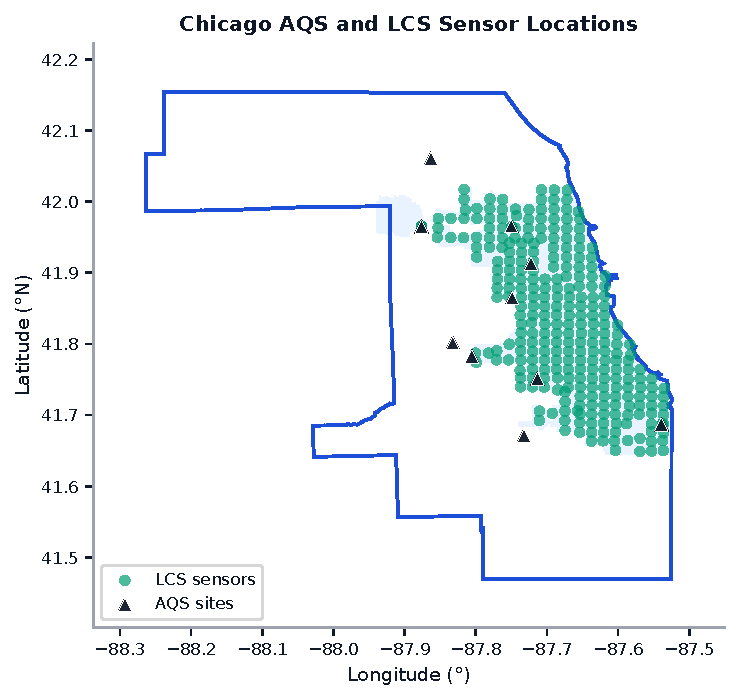
\includegraphics[width=0.85\textwidth]{Plots/Supporting_Information/Figure_SI_15/chicago_network_with_reference_monitors.pdf}
 \caption{Chicago Open Air low-cost sensor network (small markers) and EPA AQS regulatory reference monitors (large markers) within Cook County. The Open Air network covers the city core densely, with nine sensors collocated at three AQS sites (Mayfair Pump Station, Schiller Park IEPA Trailer, Washington HS); these nine collocated sensors are excluded from the primary finite-population analysis.}
 \label{fig:si_chicago_network}
\end{figure}

\begin{figure}[H]
 \centering
 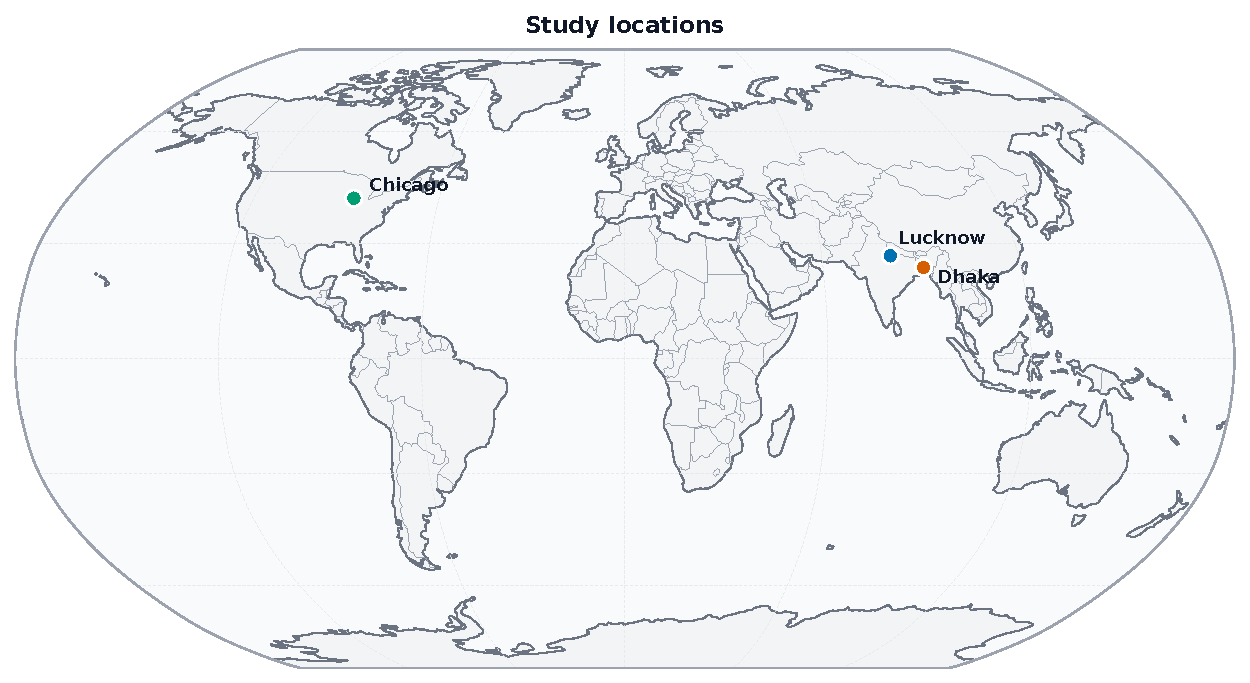
\includegraphics[width=0.85\textwidth]{Plots/Supporting_Information/Figure_SI_16/regional_locator.pdf}
 \caption{Regional locator showing the geographic context of the three sensor networks: \city{Lucknow} in the central Indo-Gangetic Plain (India), \city{Dhaka} in the lower IGP delta (Bangladesh), and \city{Chicago} on the U.S.\ Midwest shore of Lake Michigan. The two South Asian cities sit roughly on the same alluvial plain at similar latitude; Chicago is at substantially higher latitude and in a markedly different climatic and emissions regime.}
 \label{fig:si_locator}
\end{figure}

\begin{figure}[H]
 \centering
 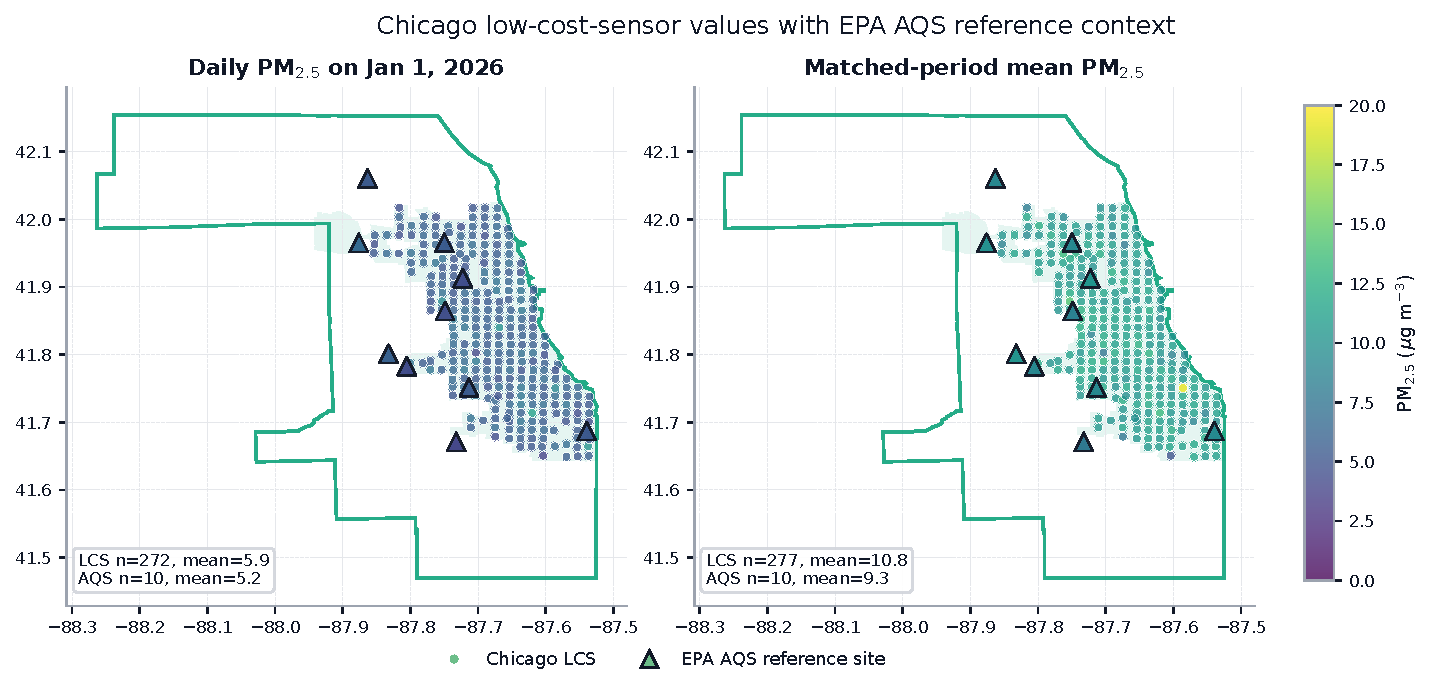
\includegraphics[width=0.95\textwidth]{Plots/Supporting_Information/Figure_SI_1/chicago_pm25_lcs_aqs_daily_period_map.pdf}
 \caption{\city{Chicago} low-cost-sensor values with EPA AQS reference context. \textbf{(left)} One-day snapshot: daily \pmtt\ on January~1, 2026 across the non-collocated Open Air low-cost sensors (circles), with EPA AQS reference sites (triangles) shown for context. \textbf{(right)} Matched valid period: September~1, 2025--March~31, 2026 mean \pmtt\ for both networks, using the period when both local daily files contain valid values. On January~1, the low-cost-network and AQS means are $5.9$ and $5.2~\units$, respectively; across the matched period the corresponding plotted site-mean averages are $10.8$ and $9.3~\units$. The AQS sites provide reference-site context only and are not the estimation target.}
 \label{fig:si_chicago_pointsample}
\end{figure}

\subsection{Missingness mechanism screens}\label{sec:si_missingness_screens}

We screened whether the day-level missingness fraction in each network is associated with concentration level, spatial variability, or temporal structure. The summarized findings are as follows. In \city{Chicago}, no association reaches even weak evidence (the strongest signal is calendar-time drift with Spearman $\rho = 0.108$, permutation $p = 0.099$). In \city{Dhaka}, the strongest associations are with daily spatial variability ($\rho = -0.133$, $p = 0.010$) and concentration ($\rho = -0.127$, $p = 0.017$), both rated as weak evidence; the negative sign indicates that high-variability and high-concentration days had \emph{lower} missingness, the opposite of what would bias the headline finding upward. In \city{Lucknow}, the strongest signal is temporal-structure drift over the deployment year ($\rho = 0.423$, $p < 0.001$, rated moderate evidence), consistent with the staggered-deployment hypothesis described in the main text. None of these tests provides evidence of a missingness mechanism that would systematically bias the reference mean toward or away from the subnetwork estimates.

\subsection{Completeness-threshold sensitivity}\label{sec:si_completeness_threshold}

We re-ran the headline Monte Carlo (10{,}000 draws) under five completeness scenarios: S0 baseline (no additional filter), S1 daily 18-hour minimum, S2 daily 12-hour minimum, S3 sensor-period 75\% retention requirement, and S5 drop sensors with any continuous gap exceeding 30 days. Results are summarized in the released analysis outputs; the key takeaway is that the sensor-count recommendations are robust across these scenarios. For example, the period MdAPE $\le 5\%$ requirement is met at $n=2$ in Chicago across all five scenarios, at $n=7$ to $n=10$ in Dhaka, and at $n=5$ to $n=20$ in Lucknow depending on filter (with the largest movement coming from the S3 75\% retention filter, which itself substantially reduces the finite population in Lucknow). The reference-mean distortion induced by the completeness filters --- which is a separate concern from sensor-count recommendation --- is small in absolute terms in Chicago and Dhaka (mean absolute difference $< 1.1$~\units\ for most scenarios), but reaches $\sim 2.6$~\units\ on average for Lucknow under the strictest filter, reflecting the genuine seasonal pattern in Lucknow's missingness rather than a measurement artifact.

\subsection{Daily $N^*$ distribution and low-coverage days}\label{sec:si_nstar_distribution}

Across the deployment year, the daily count of valid sensors $N^*$ remained at or above the largest evaluated subnetwork size ($n=30$) on essentially every day in Lucknow and Chicago. In Dhaka, a small number of days have $N^*$ below 30; daily Monte Carlo draws on such days enforce $n \le N^*$ at the subset level, and we report exclusion counts in the underlying daily summary. The lowest-coverage sensor in Lucknow reports 4.5\% uptime; the lowest-coverage Chicago sensor reports 24\% uptime. Median uptime statistics reported in Section~\ref{sec:methods} of the main text use the median rather than the mean precisely because of these long-tail outliers in the uptime distribution.

\subsection{Low-but-nonzero outlier screening}\label{sec:si_low_tail}

We also screened for low-but-nonzero outliers: values that pass the basic physical-plausibility QA/QC at $\pmtt > 0$ but appear anomalously low relative to neighboring sensors, as can occur from local sheltering or partially obstructed inlets. We ran a diagnostic screening of the lower tail of the daily sensor-mean distribution at each network. The output shows no consistent low-tail anomaly that would justify retroactive filtering: in particular, the suspect low-value patterns described in the literature (e.g., urban values $\sim 4~\units$ embedded among neighbors exceeding $100~\units$) do not appear in our networks at material rates. We retain all such values to reflect realistic operating conditions, and we list any individual sensor-day flags that did meet the diagnostic criteria in the underlying CSV.

\subsection{Diurnal feature preservation under subsampling}\label{sec:si_diurnal_preservation}

To confirm that subnetwork mean estimation does not distort diagnostic temporal features of the network signal, we tested whether random subnetworks of size $n = 5, 10, 20$ preserve the typical-day diurnal cycle of the parent network. Mean hourly profiles were computed for the full network and for random subnetwork draws at each $n$, separately for each city. The full-network diurnal patterns differ qualitatively between the three networks: in \city{Dhaka} and \city{Lucknow}, the diurnal cycle peaks in the evening (hour 21 local time) and troughs in mid-afternoon (hour 15), with amplitudes of 29.2~\units\ (54\% of the hourly mean) in \city{Dhaka} and 40.7~\units\ (66\% of the hourly mean) in \city{Lucknow} --- consistent with traffic, residential combustion, and shallow nocturnal boundary layers driving evening peaks. \city{Chicago} shows the opposite pattern, peaking in the morning (hour 8) and troughing in mid-afternoon (hour 15), with a much smaller amplitude of 2.0~\units\ (19\% of the hourly mean), consistent with a flatter pollution regime and lake-effect mixing. Across subnetwork sizes, the diurnal-cycle shape is preserved in all three cities: the relative diurnal amplitude is preserved within roughly 10\% at $n=10$ and within roughly 5\% at $n=20$, and the timing of peaks and troughs is unchanged. The key implication is that subnetwork mean estimates do not systematically distort the diurnal profile, even though the diurnal shape differs across cities. Details and per-hour profiles are in the released analysis outputs.

\subsection{LCS-vs-AQS comparison and Chicago raw-vs-calibrated sensitivity}\label{sec:si_chicago_sensitivity}

Chicago is the only network in our study with co-located regulatory reference monitors at sufficient density to support an instrument-level comparison. At the network-mean level over the 212 days when both AQS and the calibrated LCS network are available, the daily LCS network mean tracks the AQS network mean with a small positive bias of $+1.56$~\units, mean absolute error 2.12~\units, and Pearson $r = 0.902$. We interpret this agreement as supportive context for the calibration pipeline; we do not treat AQS as a truth replacement for the LCS finite-population estimand, since the AQS network is a sparse 10-site array sampling different locations than the Open Air sensors.

The raw-vs-calibrated comparison is more consequential for interpretation. The raw uncalibrated Open Air network period mean over the same evaluated daily aggregates is $17.18$~\units, versus $10.25$~\units\ for the calibrated network mean --- a shift of $+6.93$~\units\ (raw above calibrated). Despite this material difference in concentration scale, the sensor-count requirements derived from the two variants are quantitatively similar: at $n=10$ the period MdAPE is 2.81\% on the raw network versus 1.90\% on the calibrated network, and the P95 APE is 8.70\% versus 6.63\%, with similar values at $n=5$ and $n=20$. The corresponding absolute concentration errors differ in proportion: the median absolute error at $n=10$ is $0.48$~\units\ on the raw network versus $0.20$~\units\ on the calibrated network. This pattern is informative for the calibration-fidelity argument in Section~\ref{sec:assumptions}: calibration quality has a much larger effect on the absolute concentration estimate (the level itself) than on the relative-error sensor-count curve. In other words, the number of sensors needed to reproduce \emph{a} reference mean is similar across the two calibration regimes; \emph{which} reference mean is reproduced depends substantially on the calibration choice.
